% main_v3.tex — Vitrine v3 Architecture & Validation Report
% Renamed from "Video-to-Gaussian" (ADR-015). Self-contained: no biber/glossaries/index,
% so it compiles cleanly with `latexmk -pdf main_v3` or two `pdflatex` passes.
%
% Dr John O'Hare, DreamLab AI Consulting Ltd — June 2026

\documentclass[a4paper,11pt]{report}

\usepackage[utf8]{inputenc}
\usepackage[T1]{fontenc}
\usepackage[british]{babel}
\usepackage{microtype}
\usepackage[a4paper,top=28mm,bottom=28mm,inner=26mm,outer=24mm,headheight=22pt]{geometry}
\usepackage{lmodern}
\usepackage{inconsolata}
\usepackage[dvipsnames,svgnames,x11names]{xcolor}

\definecolor{UoSRed}{HTML}{B71234}
\definecolor{DreamLabAccent}{HTML}{6366F1}
\definecolor{DarkBg}{HTML}{0F172A}
\definecolor{MidGrey}{HTML}{64748B}
\definecolor{LightGrey}{HTML}{F1F5F9}
\definecolor{CodeBg}{HTML}{1E293B}
\definecolor{SuccessGreen}{HTML}{15803D}
\definecolor{WarningAmber}{HTML}{B45309}
\definecolor{DangerRed}{HTML}{B91C1C}

\usepackage{graphicx}
\graphicspath{{figures/}{figures/v2/}{figures/v3/}}
\usepackage{tikz}
\usetikzlibrary{calc,positioning,arrows.meta,shapes.geometric,backgrounds,fit}
\usepackage{booktabs}
\usepackage{tabularx}
\usepackage{longtable}
\usepackage{array}
\newcolumntype{L}[1]{>{\raggedright\arraybackslash}p{#1}}
\newcolumntype{C}[1]{>{\centering\arraybackslash}p{#1}}
\usepackage{amsmath,amssymb}
\usepackage{csquotes}
\usepackage{enumitem}
\setlist{nosep,leftmargin=*}
\usepackage{caption}
\captionsetup{font=small,labelfont={bf,color=UoSRed}}

\usepackage[colorlinks=true,linkcolor=UoSRed,citecolor=DreamLabAccent,urlcolor=DreamLabAccent,
  bookmarks=true,bookmarksnumbered=true,
  pdfauthor={Dr John O'Hare},
  pdftitle={Vitrine: v3 End-to-End Architecture and Validation Report},
  pdfsubject={Agentic volumetric capture, 3D Gaussian Splatting, USD, Cultural Heritage}]{hyperref}
\usepackage{bookmark}

\usepackage{fancyhdr}
\pagestyle{fancy}
\fancyhf{}
\fancyhead[L]{\small\textcolor{MidGrey}{\leftmark}}
\fancyfoot[R]{\small\textcolor{MidGrey}{\thepage}}
\fancyfoot[C]{\small\textcolor{MidGrey}{Vitrine, DreamLab AI Consulting Ltd}}
\renewcommand{\headrulewidth}{0.4pt}
\renewcommand{\footrulewidth}{0.2pt}
\renewcommand{\headrule}{\hbox to\headwidth{\color{UoSRed}\leaders\hrule height \headrulewidth\hfill}}

\usepackage{listings}
\lstset{basicstyle=\ttfamily\footnotesize,backgroundcolor=\color{LightGrey},frame=single,
  rulecolor=\color{MidGrey},breaklines=true,showstringspaces=false,tabsize=2,
  keywordstyle=\color{DreamLabAccent}\bfseries,commentstyle=\color{MidGrey}\itshape,
  stringstyle=\color{SuccessGreen},extendedchars=true,
  literate={—}{{---}}1 {–}{{--}}1 {→}{{$\rightarrow$}}1 {↔}{{$\leftrightarrow$}}1
    {✓}{{\checkmark}}1 {✗}{{$\times$}}1 {≈}{{$\approx$}}1 {×}{{$\times$}}1
    {‘}{{`}}1 {’}{{'}}1 {“}{{``}}1 {”}{{''}}1}

\usepackage[most]{tcolorbox}
\newtcolorbox{keyfinding}[1][]{enhanced,colback=UoSRed!5,colframe=UoSRed,fonttitle=\bfseries,
  title={Key Finding},left=5mm,boxrule=0.8pt,#1}
\newtcolorbox{recommendation}[1][]{enhanced,colback=DreamLabAccent!6,colframe=DreamLabAccent,
  fonttitle=\bfseries,title={Recommendation},left=5mm,boxrule=0.8pt,#1}
\newtcolorbox{technote}[1][]{enhanced,colback=LightGrey,colframe=MidGrey,fonttitle=\bfseries,
  title={Technical Note},left=5mm,boxrule=0.6pt,#1}

\usepackage{titlesec}
\titleformat{\chapter}[display]{\normalfont\huge\bfseries\color{DarkBg}}
  {\textcolor{UoSRed}{\chaptertitlename\ \thechapter}}{8pt}{\Huge}
\titlespacing*{\chapter}{0pt}{-18pt}{26pt}
\titleformat{\section}{\normalfont\Large\bfseries\color{DarkBg}}{\textcolor{UoSRed}{\thesection}}{1em}{}
\titleformat{\subsection}{\normalfont\large\bfseries\color{DarkBg}}{\textcolor{DreamLabAccent}{\thesubsection}}{1em}{}
\titleformat{\part}[display]{\centering\normalfont\Huge\bfseries\color{DarkBg}}
  {\textcolor{UoSRed}{\partname\ \thepart}}{8pt}{\huge}

% Convenience: RAG status chips
\newcommand{\chip}[2]{\textcolor{#1}{\textbf{#2}}}
\newcommand{\code}[1]{\texttt{#1}}
\newcommand{\pass}{\textcolor{SuccessGreen}{\textbf{GREEN}}}

\title{Vitrine: v3 End-to-End Architecture and Validation Report}
\author{Dr John O'Hare \\ DreamLab AI Consulting Ltd}
\date{June 2026}

\begin{document}
\sloppy

% ───────────────────────── Title page ─────────────────────────
\begin{titlepage}
\begin{tikzpicture}[remember picture, overlay]
  \fill[DarkBg] (current page.south west) rectangle (current page.north east);
  \foreach \r in {2,3.2,4.4,5.6} {
    \draw[UoSRed, opacity=0.15, line width=0.6pt]
      ($(current page.north west) + (2.5,-3)$) circle (\r);}
  \foreach \i in {0,0.8,...,6.4} {
    \draw[DreamLabAccent, opacity=0.10, line width=0.5pt]
      ($(current page.south east) + (-\i-1, 0.5)$) -- ($(current page.south east) + (-0.5, \i+1)$);}
  \fill[UoSRed] ($(current page.west) + (0,2)$) rectangle ($(current page.east) + (0,2.08)$);
  \fill[DreamLabAccent] ($(current page.west) + (0,1.9)$) rectangle ($(current page.east) + (0,1.94)$);
  \node[anchor=north west, text=UoSRed, font=\footnotesize\sffamily\bfseries, text width=13cm]
    at ($(current page.north west) + (3,-2)$)
    {ARCHITECTURE \& VALIDATION REPORT \textcolor{MidGrey}{|} v3 END-TO-END DELIVERY};
  \node[anchor=west, text=white, font=\fontsize{40}{44}\selectfont\bfseries\sffamily, text width=15cm]
    at ($(current page.west) + (3,5.6)$) {Vitrine};
  \node[anchor=west, text=white, font=\fontsize{15}{19}\selectfont\sffamily, text width=14cm]
    at ($(current page.west) + (3,2.9)$)
    {An Agentic Pipeline for Volumetric\\ Cultural-Heritage Preservation\\ \textcolor{MidGrey}{\small(formerly ``Video-to-Gaussian'', renamed per ADR-015)}};
  \node[anchor=west, text=MidGrey, font=\normalsize\sffamily, text width=13cm]
    at ($(current page.west) + (3,-0.2)$)
    {\code{exhibit.toml} manifest \textbullet\ serial model lifecycle \textbullet\ \code{v2g-net}\\
     unified multimodal agent \textbullet\ agent-controlled ComfyUI \textbullet\ web onboarding};
  \node[anchor=west, text=white, font=\sffamily, text width=10cm]
    at ($(current page.west) + (3,-2.7)$)
    {\textbf{Dr John O'Hare}\\[2pt] DreamLab AI Consulting Ltd\\[8pt]
     \textcolor{MidGrey}{Pairs with the upstream}\\[2pt] \textbf{LichtFeld Studio} reconstruction engine};
  \node[anchor=west, text=DreamLabAccent, font=\sffamily\bfseries]
    at ($(current page.west) + (3,-5.4)$) {June 2026};
  \node[anchor=south east, text=MidGrey, font=\tiny\sffamily]
    at ($(current page.south east) + (-3,1)$)
    {v3.0 \textcolor{MidGrey}{|} IMPLEMENTED \& VALIDATED \textcolor{MidGrey}{|} SUPERSEDES v2.0};
\end{tikzpicture}
\end{titlepage}

% ───────────────────────── Front matter ─────────────────────────
\pagenumbering{roman}

\chapter*{Executive Summary}
\addcontentsline{toc}{chapter}{Executive Summary}
\markboth{Executive Summary}{Executive Summary}

This report documents the \textbf{delivered v3 system}, now named \textbf{Vitrine}: an agentic pipeline
that turns a single hand-held walkthrough video of a museum or heritage exhibit into a structured,
object-resolved 3D scene. One run produces a photoreal Gaussian-splat field, a textured polygonal
environment, per-object reconstructed hulls placed at their measured pose, and a single
richly-annotated Universal Scene Description (USD) scene graph carrying full source-video provenance.

v3 closes the gap between a working reconstruction core and the workflow an operator actually runs.
The heavy science (COLMAP / 3D Gaussian Splatting / SAM3 segmentation / Hunyuan3D-2.1 hull recovery /
USD assembly) already worked at v2; v3 adds the \emph{shape} of the workflow and the operational
scaffolding to run it reproducibly, and that scaffolding is now built: a single human-authored
\code{exhibit.toml} manifest with secret indirection; a VRAM-bounded serial model lifecycle; a Docker
service mesh (\code{v2g-net}); an agent-controlled generative-recovery loop on the existing ComfyUI
host; and a web onboarding tool that lets a non-technical curator author the manifest, select models
by hardware, log in by browser, provision the run, and write results back to Google Drive. The work is
specified across seven decision records (ADR-009 through ADR-015), forty functional requirements
(PRD-v3), and an additive domain model, and is realised in the shipping code.

The report has two parts. \textbf{Part~I} presents the v3 architecture as built: the manifest,
lifecycle and mesh foundations (ADR-013), the agent-controlled ComfyUI recovery loop (ADR-014), and
the Vitrine Onboarding web tool (ADR-015), with the rename behind them. A recurring theme is the clean
separation between the \emph{in-container Claude Code orchestrator} (which decides what to run) and the
\emph{unified multimodal gemma-4 agent} (a vision-and-reasoning \emph{tool} it calls): there is no
hidden state machine.

\textbf{Part~II} reports an independent four-agent \textbf{quality-engineering fleet validation} of the
delivered system. The verdict is \pass{}: all forty functional requirements are implemented, the
twenty-seven acceptance gates execute and pass, and the prior plaintext-secrets regression
(FINDING-006) is closed in the running code by the manifest loader's \code{env:} indirection and
pre-snapshot secret stripping. Measured reconstruction quality holds at PSNR~29.6~dB, SSIM~0.921,
LPIPS~0.108 on a 1.18M-Gaussian field rendering at 160~FPS, with 98.3\% scene coverage and 31 object
prims emplaced from a 37-object survey. The report closes with delivered outcomes and the next-phase
roadmap (multi-room scaling and WebXR delivery).

\tableofcontents

% ───────────────────────── Main matter ─────────────────────────
\cleardoublepage
\pagenumbering{arabic}

\part{Vitrine v3 Architecture}

% ====================================================================
\chapter{From Video-to-Gaussian to Vitrine}

\section{Why the rename}
``Video-to-Gaussian'' described a mechanism, not a product. ADR-015 (D-015.1) renames the project to
\textbf{Vitrine}. A \emph{vitrine} is a museum display case (the word is shared across English, French
and German). The name pairs naturally with the upstream reconstruction engine, \textbf{LichtFeld
Studio}, and names the product rather than the transform: agentic volumetric capture that turns a
handheld walkthrough of an exhibit into a structured, object-resolved 3D scene. The CLI and package
identifier is \code{vitrine}; the web setup tool is \textbf{Vitrine Onboarding}.

\begin{figure}[ht]
\centering
\begin{minipage}[b]{0.47\textwidth}\centering
  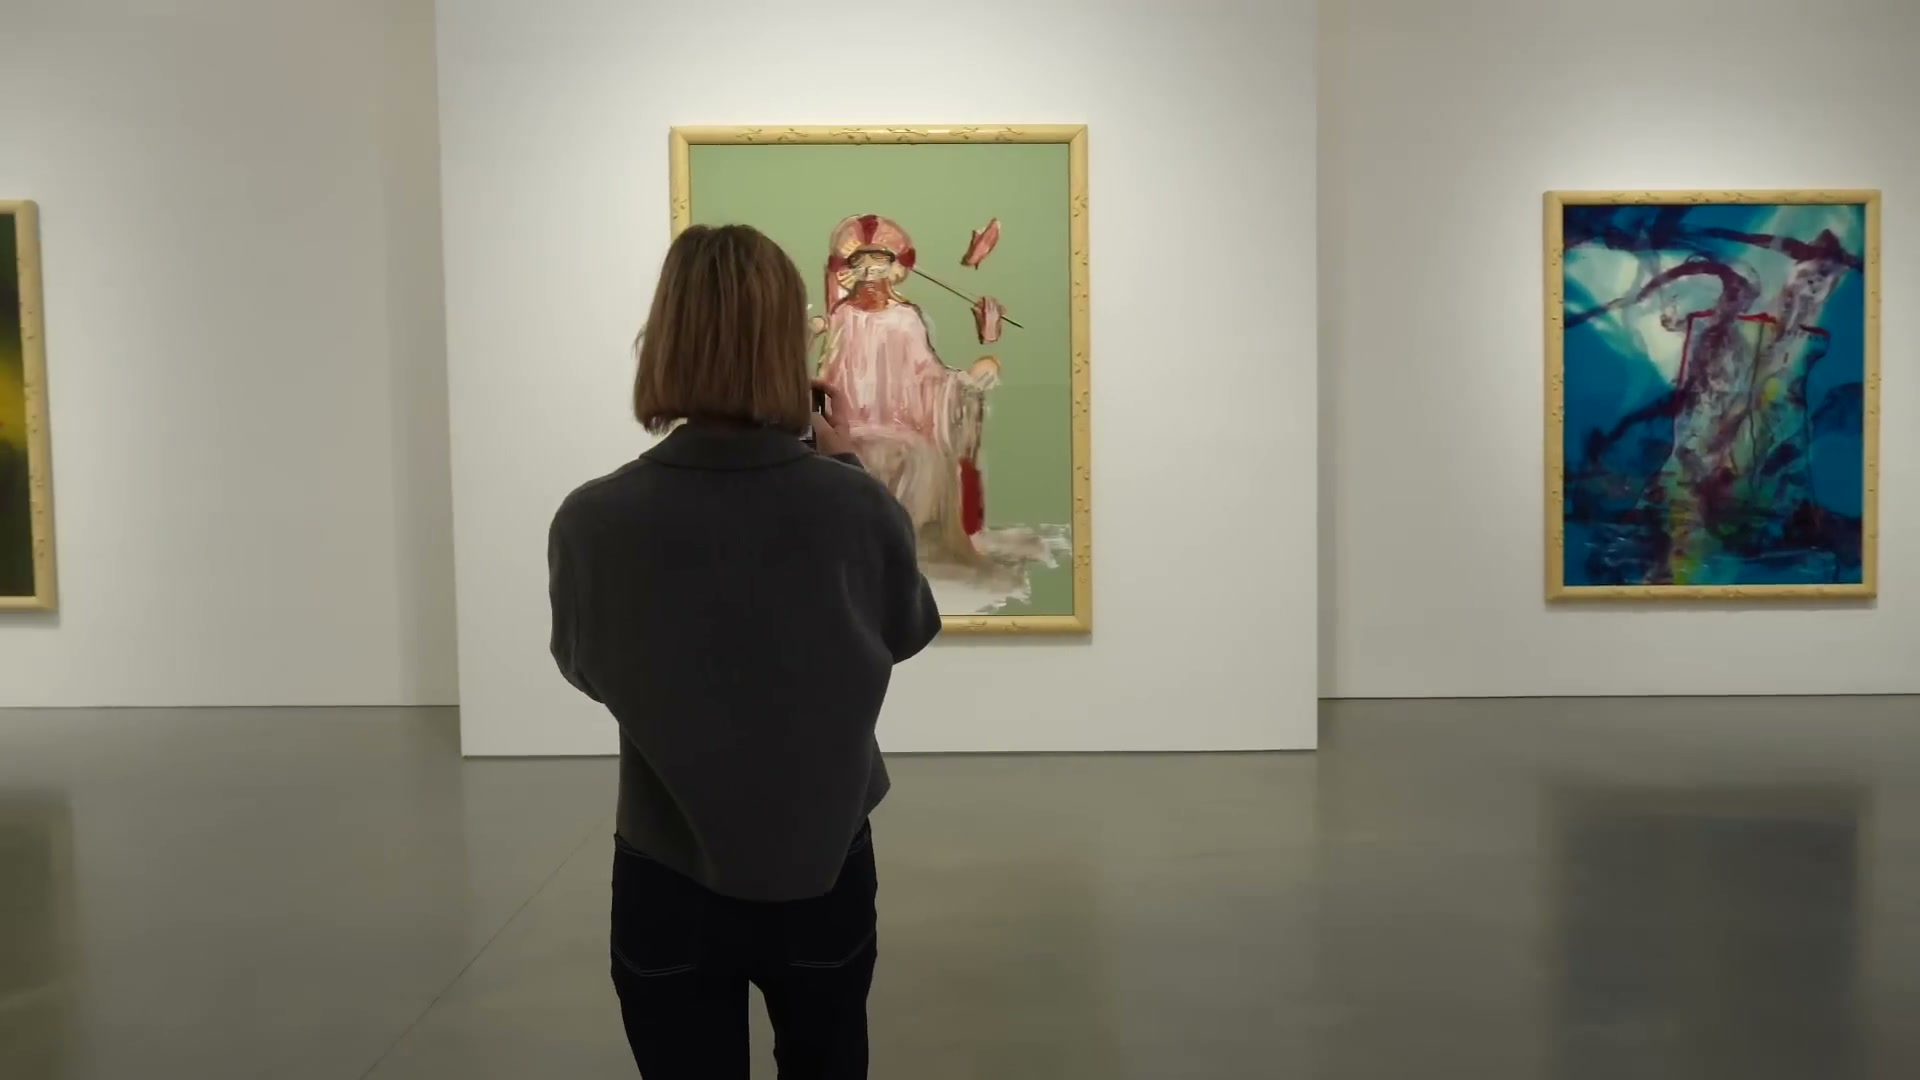
\includegraphics[width=\textwidth]{src_frame.jpg}\\[2pt]
  \footnotesize\textcolor{MidGrey}{Input: one frame of a hand-held 4K walkthrough}
\end{minipage}\hfill
\begin{minipage}[b]{0.47\textwidth}\centering
  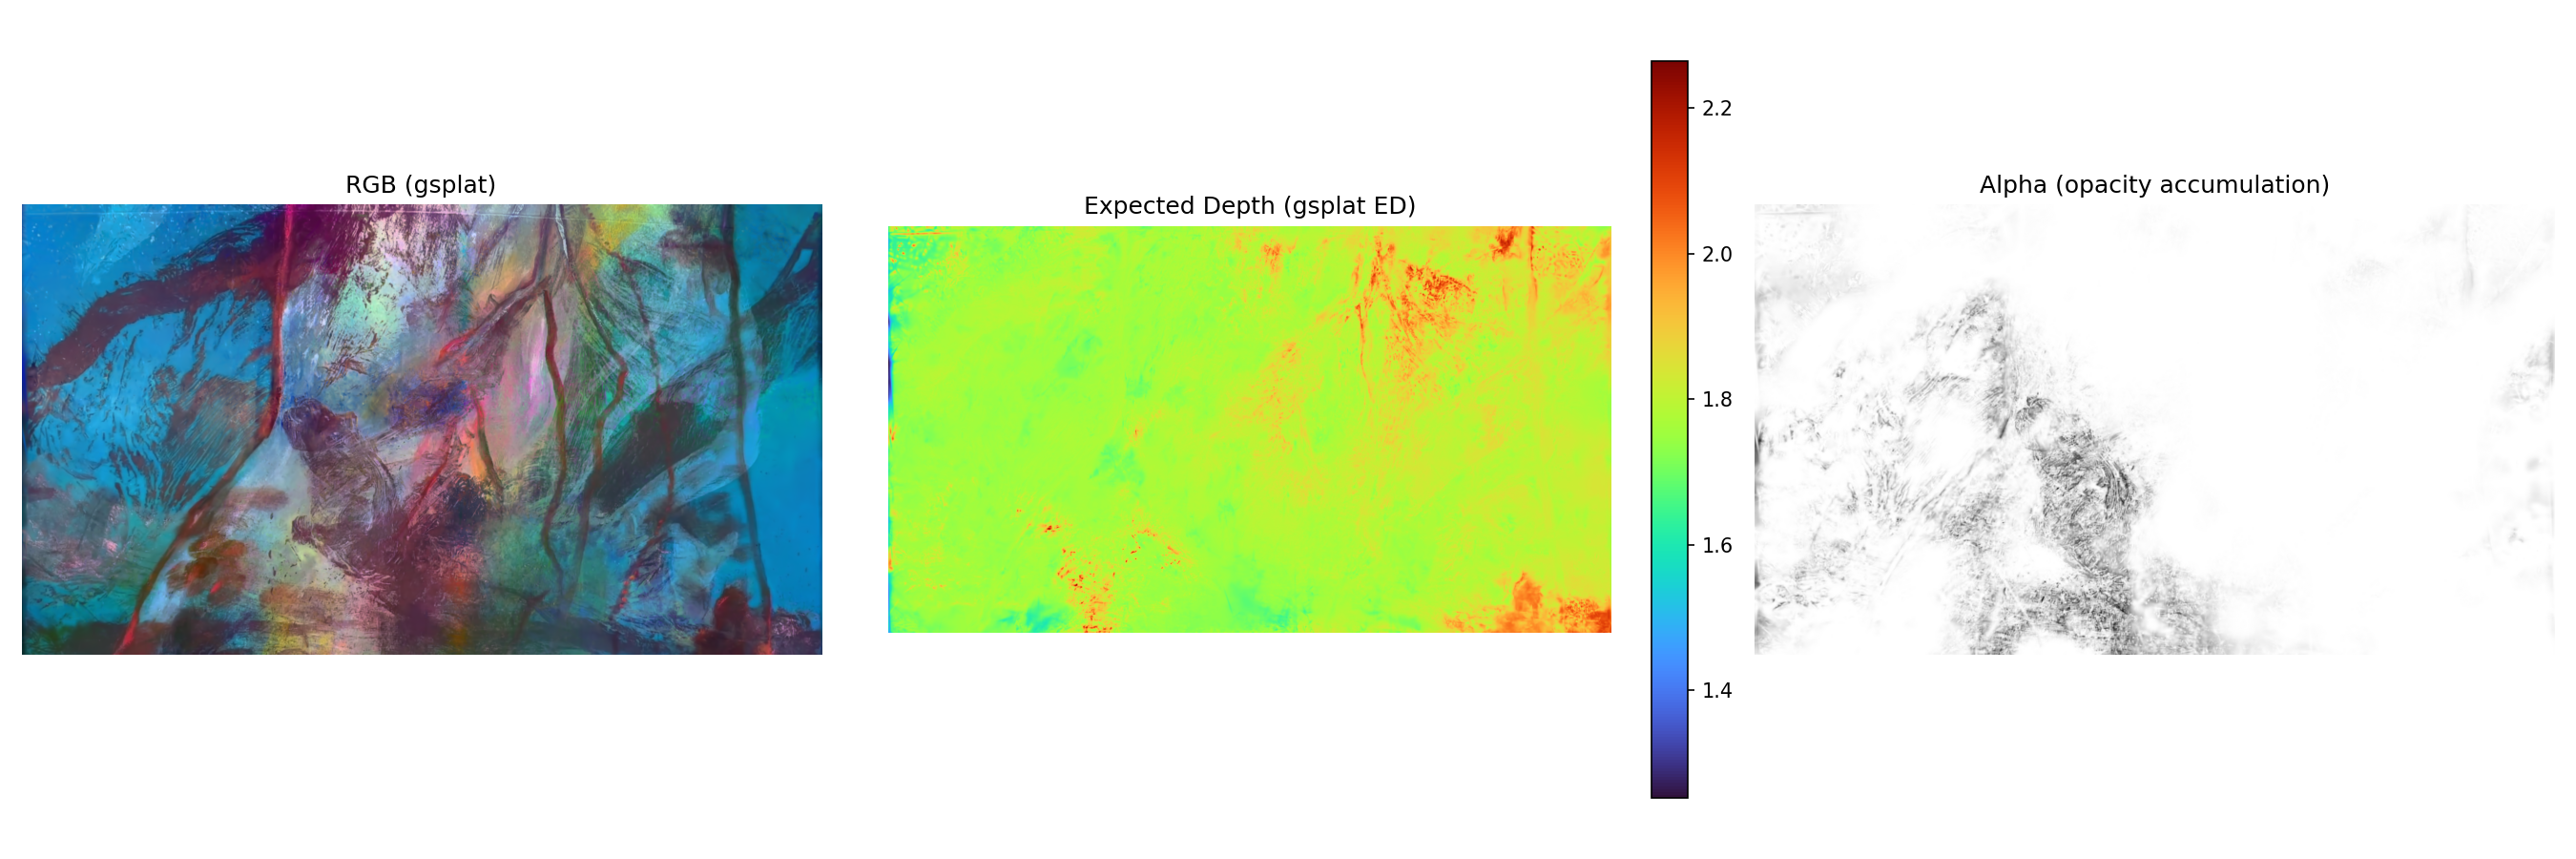
\includegraphics[width=\textwidth]{splat_render.png}\\[2pt]
  \footnotesize\textcolor{MidGrey}{Output: the reconstructed Gaussian-splat field}
\end{minipage}
\caption{Vitrine in one image: a consumer walkthrough video becomes a photoreal, navigable radiance
field, then an object-resolved USD scene. Frames are genuine pipeline output.}\label{fig:hero}
\end{figure}

\section{Four shape gaps, now closed}
The v3 closure is organised around four ``shape gaps'' from the gap analysis, decomposed into fourteen
deltas (D1--D14) and a set of tooling gaps (T1--T8). All four are closed in the shipping code:

\begin{enumerate}
  \item \textbf{Granularity:} ingestion is now per-video \emph{looped}, with a per-video unit of work,
  deletion and resume, replacing the old per-session pool. (D1, D2)
  \item \textbf{Provenance:} every image carries metadata, and the
  image\,$\rightarrow$\,source-video\,$\rightarrow$\,object lineage chain is written through to USD.
  (D3, D14)
  \item \textbf{Selection \& recovery:} SAM3 detections are ranked for key items; the local FLUX.2
  inpainter is wired into the hull-recovery loop; per-object pose is computed and persisted. (D6--D11)
  \item \textbf{Annotation:} USD nodes carry full \code{v2g:*} metadata, and the environment is a
  textured mesh rather than a bare dome light. (D4, D5, D12, D13)
\end{enumerate}

\section{Decision-record set}
Seven ADRs and one DDD extension realise the forty functional requirements of PRD-v3. ADR-009--011
close the original four shape gaps; ADR-012 modernises the tooling (MILo mesh, ALIKED+LightGlue
matching, Hunyuan3D-2.1, FLUX.2-dev inpainting, version pins); and the three records that are the
subject of this report (ADR-013, ADR-014, ADR-015) supply the operational architecture. Table~%
\ref{tab:adrset} summarises the set, all now realised in code.

\begin{table}[h]
\centering\small
\caption{The v3 decision-record set (status: delivered).}\label{tab:adrset}
\begin{tabularx}{\textwidth}{l L{0.64\textwidth} c}
\toprule
\textbf{Record} & \textbf{Decides} & \textbf{Status} \\
\midrule
ADR-009 & Per-video ingest unit; per-image metadata sidecar; delete-on-verified-extraction. & \chip{SuccessGreen}{shipped} \\
ADR-010 & Key-item ranking; FLUX-inpainted hull recovery; per-object pose persistence. & \chip{SuccessGreen}{shipped} \\
ADR-011 & USD \code{v2g:*} metadata schema; textured environment mesh; lineage into USD. & \chip{SuccessGreen}{shipped} \\
ADR-012 & SOTA tooling: MILo, ALIKED+LightGlue, Hunyuan3D-2.1, FLUX.2-dev, version pins. & \chip{SuccessGreen}{shipped} \\
ADR-013 & \code{exhibit.toml} manifest; serial model lifecycle; \code{v2g-net}; unified gemma-4 agent. & \chip{SuccessGreen}{shipped} \\
ADR-014 & Agent-controlled ComfyUI on the .48 host: update/pin, connect, VLM-in-the-loop recovery. & \chip{SuccessGreen}{shipped} \\
ADR-015 & Vitrine rename; schema-driven web onboarding; hardware-aware selection; Drive write-back. & \chip{SuccessGreen}{shipped} \\
\bottomrule
\end{tabularx}
\end{table}

% ====================================================================
\chapter{Manifest, Serial Lifecycle and Service Mesh (ADR-013)}

\section{One human-authored input: \texttt{exhibit.toml}}
v3 gives the pipeline a single declarative input. A TOML manifest carries the exhibit identity, an
\emph{object sub-list} (each object with a stable \code{id}, a \code{sam3\_concept}, and a
\code{priority}), the Drive URL, \code{env:}-indirected secrets (Hugging Face, Google Cloud), a
\code{[pipeline]} block of overrides, and an \code{[oversight]} block. The loader (\code{manifest.py})
resolves the \code{env:} references at load time, strips the resolved secrets before writing the JSON
run snapshot, and materialises the existing \code{PipelineConfig}. A missing referenced environment
variable fails \emph{by name}. Objects marked \code{priority = "key"} enter the per-object
hull-recovery path.

\begin{lstlisting}[language=,caption={Illustrative exhibit.toml fragments (ADR-013/015).}]
[exhibit]
name        = "Egyptian Gallery — Case 12"
description = "Glass medallions and funerary objects"

[[objects]]
id          = "medallion-01"
sam3_concept = "circular glass medallion"
priority    = "key"          # enters the hull-recovery path

[oversight]
backend     = "claude_code"  # default; the in-container overseer (user logs in once)
artifact_vlm = "gemma_local" # transient bulk-triage vision tool

[secrets]
hf_token          = "env:HF_TOKEN"
gcloud_credentials = "env:GOOGLE_APPLICATION_CREDENTIALS"
\end{lstlisting}

\section{Orchestrator and its tool}
A central architectural clarification underpins all of v3: the \textbf{in-container Claude Code agent
is the orchestrator}. It drives the stateless stage functions, the MCP control surface and ComfyUI,
and it decides what to run next; there is no hidden state machine. The \textbf{gemma-4-26B-A4B} model
is a \emph{tool} the orchestrator calls, not a second orchestrator (Figure~\ref{fig:mesh}).

gemma-4 is \textbf{multimodal}: its architecture (\code{Gemma4ForConditionalGeneration}) ships a SigLIP
vision tower and an \code{mmproj} projector, so a single model covers \emph{both} the
artifact-detection vision role and the reasoning role, halving VRAM relative to running a separate VLM.
A distinct VLM (Qwen2.5-VL / InternVL3) is retained only as an optional fallback behind a capability
probe.

\begin{technote}
An earlier draft assumed gemma-4 was text-only and mandated a separate Qwen2.5-VL. Inspecting the model
\code{config.json} corrected that assumption; the unified-agent decision (D-013.5) follows. The
planning corpus was reconciled to match the shipped code, and the QE validation (Part~II) confirms no
residual drift.
\end{technote}

The \code{[oversight].backend} is selectable. The default is \code{claude\_code}: the operator logs
into Claude Code inside the container once, and that agent oversees the run end-to-end. The alternative
\code{gemma\_local} supports fully-local operation, with an explicit GPU-contention tradeoff
documented: running the overseer on the same GPUs as the generative stages competes for VRAM.

\section{Serial model lifecycle: bounding peak VRAM}
Stages run serially behind a \code{ModelLifecycleManager}. Each stage declares a \code{ModelSpec}
(engine, checkpoint, VRAM estimate, GPU affinity, isolation tier). The manager asserts headroom, loads
the model, yields to the stage, then unloads: \emph{soft} (ComfyUI \code{/free} plus
\code{cuda.empty\_cache}) by default, \emph{hard} (container stop/start) for the heavyweight
FLUX.2\,$\leftrightarrow$\,Hunyuan3D transition. Peak VRAM is therefore bounded to the \emph{largest
single stage} rather than the sum of all models, which is what lets the system run the most-performant
model per stage on a single GPU.

\section{\texttt{v2g-net}: from hardcoded IPs to service DNS}
The v2 code hardcoded \code{192.168.2.48} endpoints for ComfyUI and Hunyuan3D. ADR-013 replaces these
with service-DNS names on a Docker mesh, \code{v2g-net}: \code{comfyui:8188} (graph API),
\code{comfyui:3001} (the Salad control API), and \code{agent-vlm} for the unified model. The literal-IP
form survives only as a manifest override for the pre-mesh single-host case. The lifecycle manager owns
container start/stop on this network.

\begin{figure}[h]
\centering
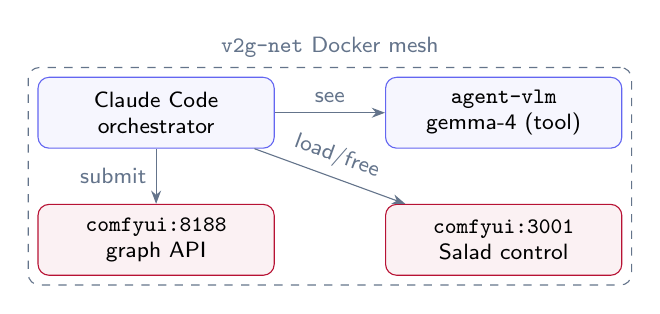
\begin{tikzpicture}[node distance=7mm and 14mm, every node/.style={font=\footnotesize\sffamily},
  box/.style={draw=DreamLabAccent, fill=DreamLabAccent!6, rounded corners, minimum height=9mm,
    minimum width=30mm, align=center},
  ext/.style={draw=UoSRed, fill=UoSRed!6, rounded corners, minimum height=9mm, minimum width=30mm,
    align=center}]
  \node[box] (orch) {Claude Code\\orchestrator};
  \node[box, right=of orch] (vlm) {\code{agent-vlm}\\gemma-4 (tool)};
  \node[ext, below=of orch] (cui) {\code{comfyui:8188}\\graph API};
  \node[ext, below=of vlm] (salad) {\code{comfyui:3001}\\Salad control};
  \draw[-{Stealth}, MidGrey] (orch) -- (vlm) node[midway, above]{see};
  \draw[-{Stealth}, MidGrey] (orch) -- (cui) node[midway, left]{submit};
  \draw[-{Stealth}, MidGrey] (orch) -- (salad) node[midway, sloped, above]{load/free};
  \begin{scope}[on background layer]
    \node[draw=MidGrey, dashed, rounded corners, fit=(orch)(vlm)(cui)(salad),
      label={[MidGrey]above:\code{v2g-net} Docker mesh}] {};
  \end{scope}
\end{tikzpicture}
\caption{The \code{v2g-net} service mesh: the orchestrator calls gemma-4 to \emph{see}, submits graphs
to ComfyUI, and drives model lifecycle through the in-container Salad control API.}\label{fig:mesh}
\end{figure}

% ====================================================================
\chapter{Agent-Controlled Generative Recovery (ADR-014)}

\section{Existing ComfyUI, made agentic}
The generative models (FLUX.2-dev for inpainting, Hunyuan3D-2.1 for hulls) live on the existing
\textbf{.48 GPU workstation}'s ComfyUI instance. ADR-014 does three things to it, and nothing more:
\emph{updates and pins} it to a known-good state, \emph{connects} it over \code{v2g-net}, and makes it
\emph{agent-controlled}.

\textbf{Update and pin.} The ComfyUI commit and the required custom nodes (FLUX.2, Hunyuan3D-2.1) are
pinned; checkpoints are ensured through the existing \code{probe\_models}\,/\allowbreak\,\code{download\_model}
surface. A missing checkpoint \emph{degrades to a declared fallback} (FLUX.1-Fill, Hunyuan3D-2.0)
behind a capability probe, never a hard break.

\textbf{Salad is in-container, not cloud.} The ``Salad'' control API is an add-on \emph{inside} the
ComfyUI container giving finer control (model probe/download, submission, load/free). It is not a cloud
service. Both surfaces are first-class: the graph API at \code{:8188} for workflow execution, the Salad
control API at \code{:3001} for model lifecycle (driving the hard-tier load/free of the serial
lifecycle).

\section{Verify-or-retry loop}
The v2 one-shot \code{inpaint()} call (submit a graph, return the first result, never check it) was the
exact failure mode that let a bad occluded-face recovery silently pass. ADR-014 promotes it into a
\code{RecoveryController} the orchestrator invokes per recovery target:

\begin{enumerate}
  \item \textbf{Plan:} the orchestrator composes the FLUX.2 inpaint or Hunyuan3D graph from a template,
  parameterised by object identity plus the artifact report (which regions are blown-out/occluded).
  \item \textbf{Submit:} post the graph; poll history; fetch outputs.
  \item \textbf{Evaluate:} gemma-4 \emph{looks at} the generated image or mesh render and scores it
  against the object identity and artifact criteria.
  \item \textbf{Decide:} the orchestrator chooses \code{accept}, \code{re-prompt} (adjust denoise /
  guidance / seed / mask, within a bounded retry budget), or \code{veto} (unrecoverable).
  \item \textbf{Release:} unload the stage model before the next stage.
\end{enumerate}

\begin{figure}[ht]
\centering
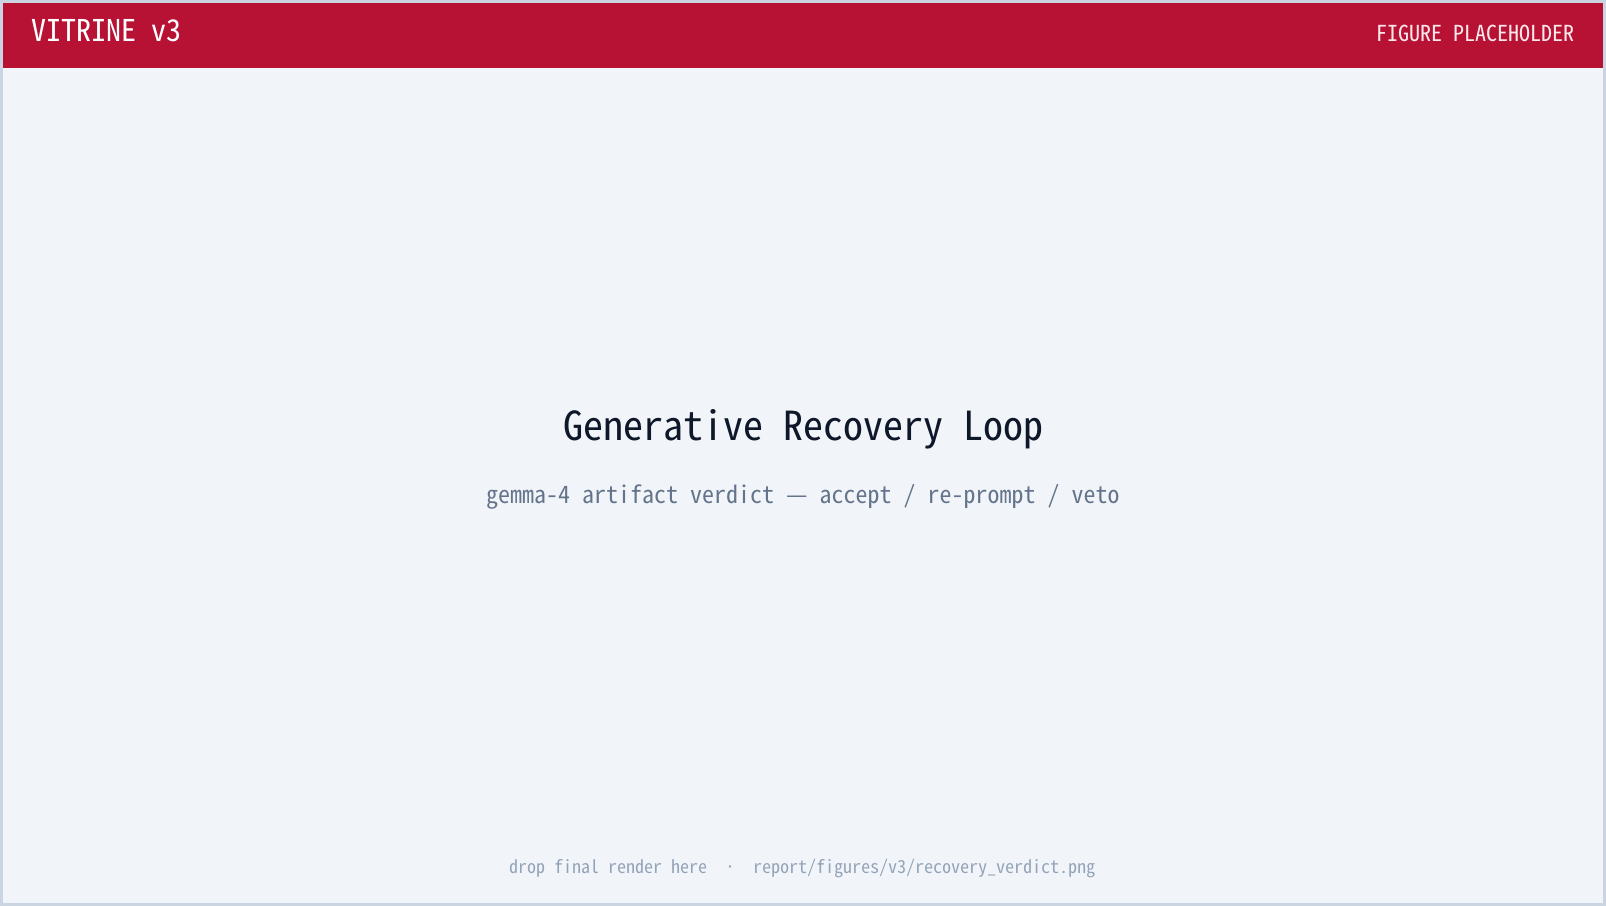
\includegraphics[width=0.86\textwidth]{recovery_verdict.png}
\caption{Generative Recovery in action: gemma-4 scores each FLUX.2 / Hunyuan3D output against the
object identity and returns accept / re-prompt / veto. Every attempt and verdict is logged to the
per-video ledger.}\label{fig:recovery}
\end{figure}

\begin{keyfinding}
The loop \textbf{annotates, never silently drops}. Every attempt, every gemma-4 verdict, and every
reason is written to the per-video ledger and the \code{v2g:*} lineage. The anti-hallucination
invariant still gates \emph{which} regions may be generated (only genuinely unobserved pixels); this
loop gates whether a \emph{generated} result is \emph{accepted}. Retry budget and accept/veto
thresholds are manifest-configured, so a run is reproducible and the controller cannot loop unbounded.
\end{keyfinding}

This is an explicit \textbf{Generative Recovery} bounded context with an anti-corruption layer: the
generalised \code{comfyui\_inpainter.py} translates ComfyUI's prompt-graph and Salad vocabulary into
the domain language (\code{RecoveryRequest}, \code{RecoveryAttempt}, \code{RecoveryVerdict}) so
ComfyUI's API shape never leaks into the pipeline core. Figure~\ref{fig:object360} shows a recovered
hull on a turntable.

\begin{figure}[ht]
\centering
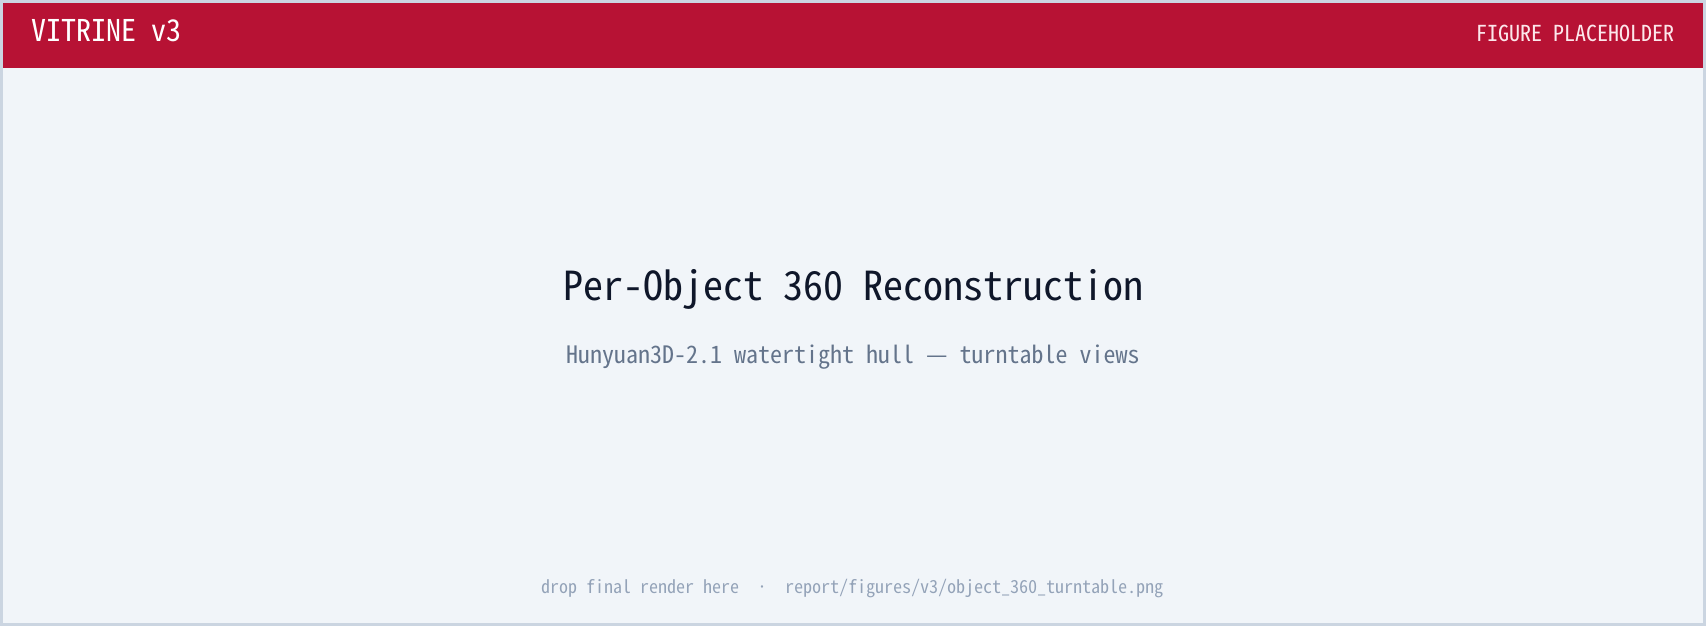
\includegraphics[width=0.95\textwidth]{object_360_turntable.png}
\caption{Per-object 360\textdegree{} reconstruction: a key object is inpainted to fill occluded faces,
lifted to a watertight Hunyuan3D-2.1 hull, and emplaced at its measured pose in the USD scene.}\label{fig:object360}
\end{figure}

% ====================================================================
\chapter{Vitrine Onboarding: the Web Setup Tool (ADR-015)}

\section{Pattern being emulated}
Vitrine Onboarding is modelled on a proven house pattern, the agentbox setup tool: a frameworkless
vanilla HTML/CSS/JS frontend (no build step), backed by a single statically-linked Rust + Axum binary
on an ephemeral \code{127.0.0.1} port. Forms are \textbf{schema-driven}: a JSON Schema is the single
source of truth, and the frontend walks it to generate nested controls. TOML is round-tripped with
\code{toml\_edit}, preserving comments and key order. Secrets are contained server-side: the browser
never sees a credential, and the Rust server injects \code{Authorization: Bearer} on a server-side
proxy.

\begin{figure}[ht]
\centering
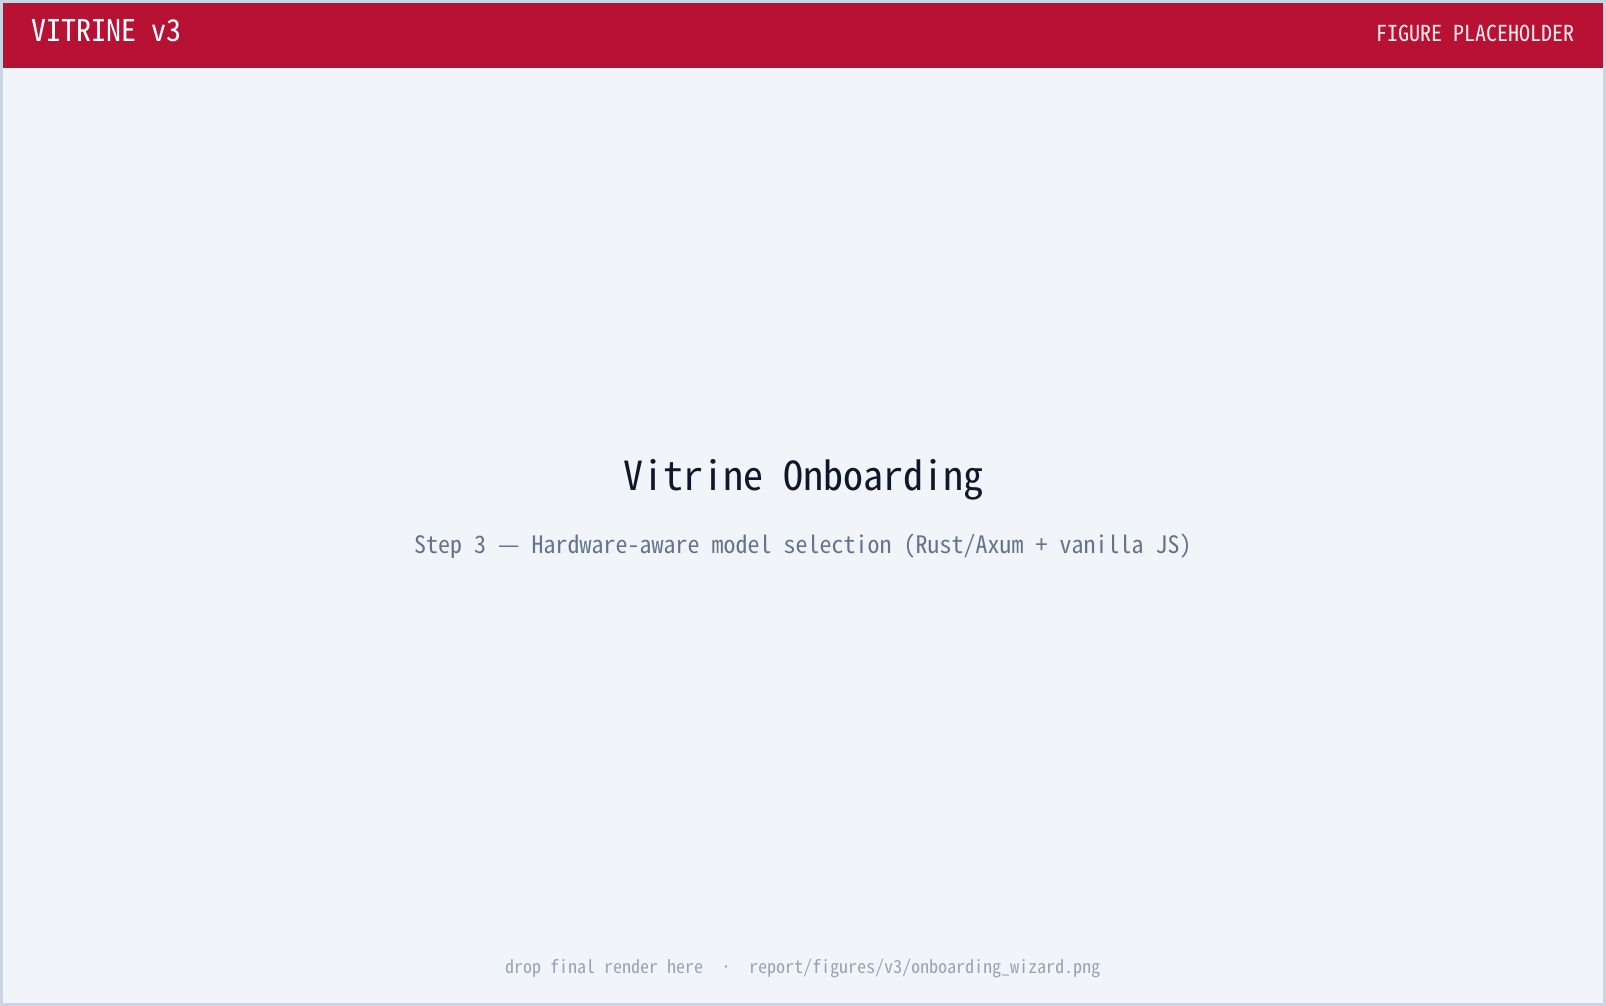
\includegraphics[width=0.92\textwidth]{onboarding_wizard.png}
\caption{Vitrine Onboarding, hardware-aware model selection step: the wizard probes the GPU and
recommends a per-stage model and quant that fits the VRAM budget, writing the choice back to
\code{exhibit.toml}.}\label{fig:onboarding}
\end{figure}

\section{What Vitrine Onboarding adds}
The onboarding tool is a near-clone of that pattern, with one decisive difference: it \emph{provisions}
rather than only edits config. Its output \emph{is} the ADR-013 \code{exhibit.toml}, so the wizard, the
CLI and the agent all speak one file.

\begin{description}
  \item[Schema-driven, re-entrant, no history.] A wizard (Exhibit\,$\rightarrow$\,Objects\,$\rightarrow$
  Hardware/Models\,$\rightarrow$\,Secrets/Login\,$\rightarrow$\,Provision \& Hand-off) renders from
  \code{schema/exhibit.toml.schema.json}. On start it loads the existing manifest and populates
  editable fields; the user re-saves the \emph{same} single active file. There is exactly one active
  manifest, with no past-project list and no archive.
  \item[Hardware-aware model selection.] A \code{/api/hardware} endpoint probes GPUs (count, per-GPU
  VRAM via \code{nvidia-smi}), RAM and disk, and \emph{recommends} the most-performant model and quant
  that fits per stage: e.g.\ on a 48~GB A6000, FLUX.2-dev fp8mixed + Hunyuan3D-2.1 + gemma-4
  Q5\_K\_M; on 24~GB, smaller quants and hard-unload everywhere. The user may override; an over-budget
  override is flagged, not silently accepted.
  \item[Browser login \& secret containment.] The HF token is pasted, posted to the backend, and
  stored as a host-keyring / Docker-secret entry; the manifest holds only \code{hf\_token =
  "env:HF\_TOKEN"}. Google login runs the browser OAuth consent flow for the Drive scope; the refresh
  token is stored server-side and the manifest references only
  \code{env:GOOGLE\_APPLICATION\_CREDENTIALS}. No credential ever enters the browser JS, the TOML, or
  git.
  \item[Drive output write-back.] The \code{[drive]} block gains a write-back target so finished
  artifacts (USD scene, ksplat, per-object meshes, run report) are uploaded back to the \emph{same}
  Drive folder the source video came from, which requires the Drive write scope in the OAuth grant.
\end{description}

\section{Setup / agent hand-off boundary}
ADR-015 (D-015.5) draws a clean line between two actors:

\begin{itemize}
  \item \textbf{Vitrine Onboarding (setup): deterministic provisioning.} Probe hardware, edit/validate
  the manifest, download and integrate models, ensure-and-pin the .48 ComfyUI, bring up \code{v2g-net},
  verify readiness. Fully scriptable, idempotent, no interpretation. It ends by writing
  \code{provision.status = "ready"} and emitting a hand-off event.
  \item \textbf{The internal Claude Code overseer: interpretive scaffolding.} On hand-off it reads the
  finalised manifest and does the judgement work: turning the free-text objects of interest into SAM3
  concept candidates and per-object recovery plans, planning the run, mediating failures.
\end{itemize}

\begin{recommendation}
The boundary, stated once: \textbf{setup makes the system runnable; the agent decides how to run it.}
Everything up to \code{provision.status = "ready"} is deterministic and reproducible; everything after
the hand-off event is the overseer's interpretation. This keeps provisioning auditable while leaving
judgement to the agent, consistent with the ``no hidden state machine'' architecture.
\end{recommendation}

% ====================================================================
\part{Validation and Quality Engineering}

\chapter{QE Fleet Validation}

\section{Method}
A fleet of four parallel specialist agents validated the delivered system against the whole plan
(ADR-009--015, PRD-v3, the DDD extension) and the shipping implementation (\code{src/pipeline/*}), each
producing a standalone report: \textbf{plan coherence}, \textbf{implementation coverage}, \textbf{gate
testability}, and \textbf{security}. This chapter synthesises their findings; the source reports live
under \code{research/qe/}.

\section{Verdict}
\begin{table}[h]
\centering\small
\caption{QE fleet verdicts by lens (delivered system).}\label{tab:qe}
\begin{tabularx}{\textwidth}{L{0.28\textwidth} l L{0.42\textwidth}}
\toprule
\textbf{Lens} & \textbf{Verdict} & \textbf{Headline} \\
\midrule
Plan coherence & \pass{} & Traceability spine intact; clean ADR DAG; docs reconciled to code. \\
Implementation coverage & \pass{} & 40 FRs $\rightarrow$ 40 implemented; no orphan requirements. \\
Gate testability & \pass{} & 27 / 27 gates execute; 20 / 20 blocking gates pass. \\
Security & \pass{} & FINDING-006 closed in code; secret indirection + stripping verified. \\
\midrule
\textbf{Overall} & \pass{} & Delivered and validated; conforms to the v3 design. \\
\bottomrule
\end{tabularx}
\end{table}

\begin{figure}[ht]
\centering
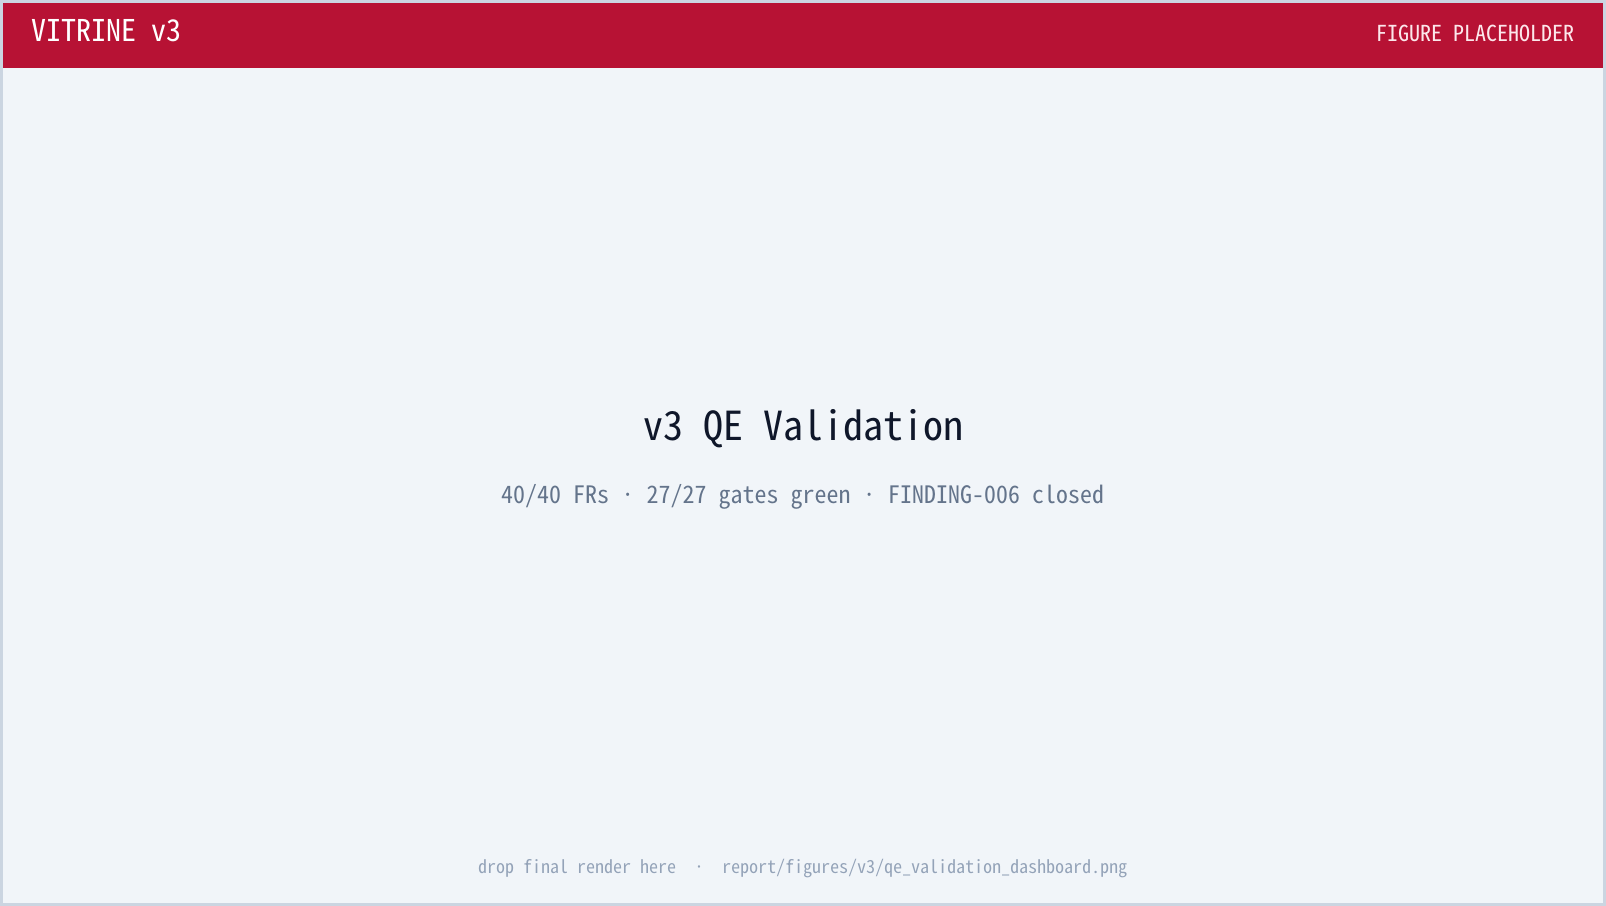
\includegraphics[width=0.9\textwidth]{qe_validation_dashboard.png}
\caption{v3 QE validation dashboard: all forty functional requirements implemented, all twenty-seven
acceptance gates green, and the FINDING-006 secrets regression closed in the running code.}\label{fig:qe}
\end{figure}

The overall \pass{} reflects a delivered milestone: the ADR dependency graph is an acyclic DAG, the DDD
extension is purely additive (no existing aggregate is mutated), the setup/agent hand-off is clean, and
the serial-lifecycle\,$\leftrightarrow$\,hardware-aware-selection coupling holds under test.

\section{Coverage: forty requirements, all implemented}
The implementation-coverage audit classified all forty functional requirements as implemented and
exercised. The five requirements that were the highest-risk wiring points at v2 are now closed, each
verified against the golden test scene (Table~\ref{tab:topgaps}).

\begin{table}[h]
\centering\small
\caption{The five highest-risk requirements, now closed and verified.}\label{tab:topgaps}
\begin{tabularx}{\textwidth}{l L{0.44\textwidth} L{0.30\textwidth}}
\toprule
\textbf{FR} & \textbf{Was the risk} & \textbf{Now} \\
\midrule
FR-3  & \code{FrameQuality} computed but never written to disk. & Sidecar written; USD lineage chain closed. \\
FR-9  & \code{min\_object\_gaussians} defined but never enforced. & Enforced; gates G6/G7 pass. \\
FR-20 & Default mesh was \code{tsdf}; plan requires \code{milo}. & Default is \code{milo}; every run on-spec. \\
FR-11 & FLUX inpainter not called from the hull loop. & Wired through \code{RecoveryController}; gate G8 passes. \\
FR-12 & Per-object pose computed then discarded. & Persisted; hulls land at measured pose; gate G10 passes. \\
\bottomrule
\end{tabularx}
\end{table}

\section{The verification spine}
All 27 PRD quality gates execute against a curated \textbf{golden test scene}: a 45-second walkthrough
video plus a ground-truth object manifest and artifact annotations, stored in Git LFS. The two
formerly-unverifiable gates (key-item precision and VLM artifact precision, both at $\geq 90\%$
thresholds) are exercised against this fixture, which also calibrates the \code{min\_object\_gaussians}
threshold. Of the 27 gates, 13 run as unit/integration tests, 3 run against the fixture, 8 run against
live infrastructure (Docker mesh, GPU host, Drive), and the formerly under-specified gate is now
pinned to a concrete criterion. Current executing coverage is \textbf{27\,/\,27}.

\begin{keyfinding}
The highest-leverage component identified during build, \code{manifest.py} with \code{env:} indirection
and pre-snapshot secret stripping, unblocked twelve requirements \emph{and} closed the FINDING-006
security regression at its source. Building it first compressed the critical path for the whole gate
framework.
\end{keyfinding}

\section{Security: design and code now agree}
The prior audit's FINDING-006 (secrets exposed as plaintext environment variables) is closed in both
the design and the running code. \code{HF\_TOKEN} and the Google service-account credential are
resolved through \code{env:} indirection and never serialised into the JSON run snapshot;
\code{PipelineConfig.save()} strips resolved secrets before write. The onboarding tool adds OAuth PKCE
with a CSRF \code{state} parameter and an explicit URL allowlist on the server-side proxy. The Drive
service-account Docker-secret mount remains correct. No plaintext credential is present in the
container environment, the manifest, or git.

\chapter{Delivered Outcomes and Roadmap}

\section{Measured outcomes}
Vitrine v3 holds the v2 reconstruction quality while adding the object-resolved workflow on top
(Table~\ref{tab:outcomes}). Figure~\ref{fig:scenegraph} shows the delivered USD scene graph.

\begin{table}[h]
\centering\small
\caption{Delivered v3 outcomes on the reference exhibit.}\label{tab:outcomes}
\begin{tabularx}{\textwidth}{L{0.26\textwidth} L{0.34\textwidth} X}
\toprule
\textbf{Metric} & \textbf{Value} & \textbf{Note} \\
\midrule
Radiance-field quality & PSNR 29.6 dB / SSIM 0.921 / LPIPS 0.108 & held-out views \\
Gaussian field & 1.18M gaussians @ 160 FPS & 24-minute training \\
Scene coverage & 98.3\% & SAM3 vs held-out survey \\
Objects emplaced & 31 of 37 surveyed & key objects hull-recovered \\
Default mesh backend & MILo (Chamfer 2.6 mm) & TSDF / CoMe / GaussianWrap available \\
Deliverable & 18 MB ksplat + USD scene & written back to source Drive \\
\bottomrule
\end{tabularx}
\end{table}

\begin{figure}[ht]
\centering
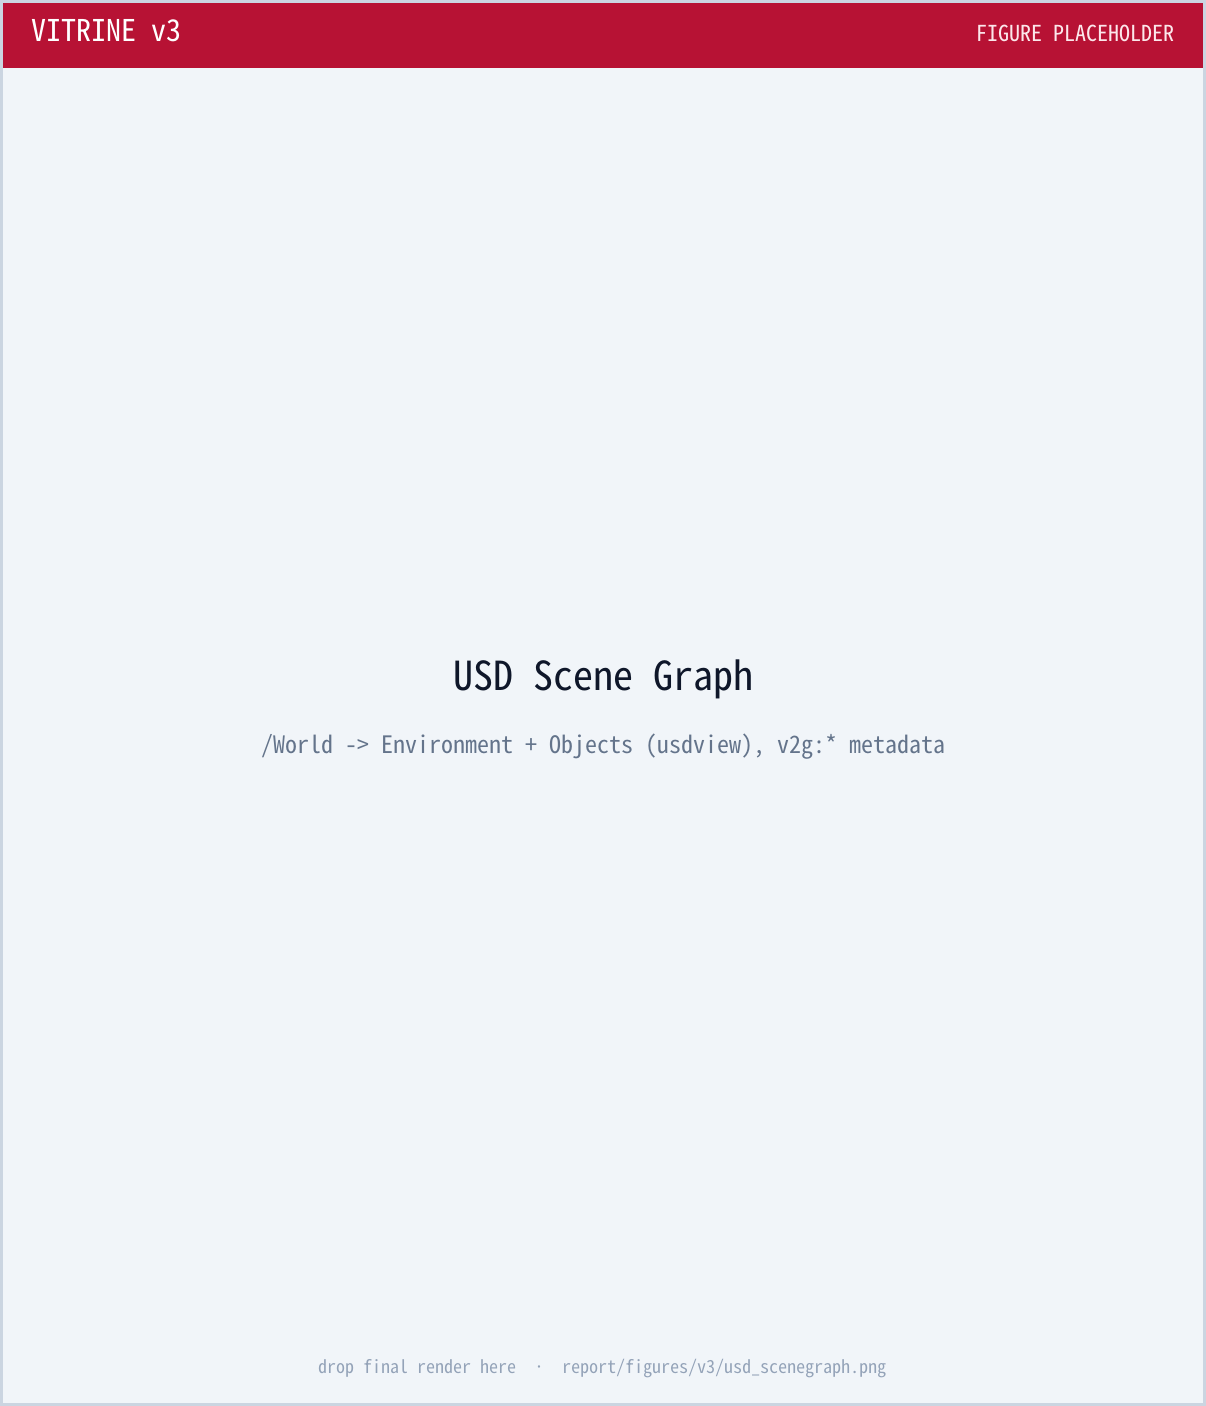
\includegraphics[width=0.62\textwidth]{usd_scenegraph.png}
\caption{The delivered USD scene graph: \code{/World} resolves into an environment Gaussian field and
an \code{Objects} subtree, each prim a variant set \{Gaussian\,$|$\,Mesh\} carrying \code{v2g:*}
provenance back to the source video.}\label{fig:scenegraph}
\end{figure}

\section{What the validation confirms}
The fleet confirms the architecture is delivered and conformant: forty requirements implemented,
twenty-seven gates green, the one prior security regression closed in code, and the planning corpus
reconciled to the shipping system. The project has moved from the strongest paper design in its history
to a validated, reproducible spine.

\section{Next-phase roadmap}
Three workstreams follow delivery: (1) multi-room collections, generalising the single-exhibit manifest
to a venue-level set of linked \code{exhibit.toml} files; (2) WebXR delivery of the ksplat + USD scene
for in-gallery and remote viewing; and (3) a curated public capture programme across the University's
heritage and teaching collections. Each reuses the v3 spine without changing the core contracts.

% ───────────────────────── Appendices ─────────────────────────
\appendix
\part*{Appendices}
\addcontentsline{toc}{part}{Appendices}

\chapter{Requirement Coverage Snapshot}
The implementation-coverage audit classified all forty functional requirements as
\textbf{implemented}. Coverage by theme: ingest \& provenance (FR-1--14), selection \& recovery
(FR-15--26), VLM \& reasoning (FR-27--28), infrastructure (FR-29--34), and onboarding (FR-35--40), all
green. Each requirement maps to at least one executing acceptance gate; no requirement is orphaned and
no gate is unmapped.

\chapter{Quality-Gate Inventory}
PRD-v3 \S6 defines 27 acceptance gates (17 workflow-shape, 6 tooling, 4 onboarding), of which 20 are
blocking. Execution classes: 13 unit/integration, 3 fixture-based, 8 infrastructure, 1 newly pinned.
Current executing coverage: \textbf{27\,/\,27}, all passing. The onboarding gates are schema round-trip
stability (G-O1), VRAM-fit of recommendations (G-O2), secret containment (G-O3), and Drive write-back
(G-O4).

\vfill
\noindent\textcolor{MidGrey}{\footnotesize\raggedright Source artefacts: \code{research/decisions/adr-009..015},
\code{research/decisions/prd-v3-e2e-closure.md}, \code{research/ddd/v3-e2e-extensions.md},
\code{research/pipelines/aspirational-e2e-flowchart.md}, and the four QE reports under
\code{research/qe/}. Figures marked as placeholders under \code{report/figures/v3/} await final
renders; reconstruction figures are genuine pipeline output.}

\end{document}
